\documentclass{scrartcl}
\usepackage[utf8]{inputenc}

\title{Threads of Ancestry and Community / Complex Threading}
\subtitle{Principia Textilica : Project Documentation}
\author{Felicitas Höbelt}
%\date{März 2015}

\usepackage{natbib}
\usepackage{graphicx}
\usepackage{caption}
\usepackage{subcaption}
\usepackage{multirow}
%\usepackage{longtable}
%\usepackage{listings}
%here goes the settings for the formatting code-section, I just leave Matlab in as an example
%\lstset{language=Matlab, basicstyle=\footnotesize,
%keywords={break,case,catch,continue,else,elseif,end,for,function,
%global,if,otherwise,persistent,return,switch,try,while,ones,zeros}}
\graphicspath{ {./img/} }


\begin{document}

\maketitle

\section{Principia Textilica}

\subsection{Context}
In the course "Principia Textilica" we explored intersections of computational algorithms and textile craft, including pattern generation algorithms, weaving techniques, knot theory, hands-on experience with textile maschines, history lessons and more.
For the final project each student was encouraged to find a subject to implement some of the methods and techniques we got to see during the course.

\subsection{Motivation}

I study Computer Science and Media, which means my background is more algorithmic/technical than art-related.
Nevertheless I am familiar with a few textile techniques such as knotting (Macramé), weaving, sewing, felting and embroidery.\\
For inspiration I looked at two topics that have fascinated me for years: Modeling "Living" Things (plants/fungi/insects/animals) and complexity.\\
Complexity is often mistaken for complicatedness because the result looks complicated.
However, the system that produces a complex result is itself very simple. It consists of a certain number of elements and a few elemantary rules which are applied to those elements.\\
My goal was to use both, complexity and modeling simple "life", to create a (textile) pattern.

\section{Idea}

\subsection{The Pond/Fish Tank}
I decided to go with a swarm model, which means I have a number of individuals which are controlled by a set of rules concerning themselves, their dynamic environment (e.g. the other members of the swarm) and their static environment (e.g. boundaries of the tank).
The metaphor I chose was a school of fish moving around in a pond or glass tank.

The desired pattern would be generated by the movements of the individuals. I wanted to start with the rules and continuously adapt them depending on the outcome.\\
I did not settle for a specific textile technique, at this point I only thought about assigning each of the individuals a thread. With this premise in mind, favourable textile techniques were embroidery and knotting.


\subsection{Rules}

My fish program is in 2D and has two main elements: the tank and the fish.\\

The tank started out as rectangular, but I found a circle to be more aesthetically pleasing as well as more fitting for an embroidery hoop. The circle embodies the simple inside/outside world that I need.

The swarm rules below share some similarities with the "Boids" program by Craig Reynolds [TODO ref], he developed an agent-based algorithm to simulate the flocking behaviour of birds.\\

The behaviour of the fish is mainly determined by four principles:\\
I Company - Each fish will follow other fish.\\
II Privacy - Each fish needs a minimum of private space.\\
III Security - Each (non-predatory) fish will avoid any predators.\\
IV Boundary - Each fish will stay inside the tank.\\

There is no randomness in my program.

\section{Implementation}
%\subsection{Unused Parameters}

For implementing my idea I chose Processing 2.0 [TODO link/ref], because I am already familiar with Java. Additionally, Processing is one of the tools we got to try out during the course, so all participants know how to look into my code and adapt it if they want to.\\

In this section I will focus more on algorithms and data flow rather than implementation details.
There are four ways of running the program represented by the combination of mechanisms that are used on top of the basic behavioural rules (predator/fear and birth/death):
1. both predator/fear and birth/death
2. only predator/fear
3. only birth/death
4. none of them

It is worth noting that the code still includes all methods and parameters that I ended up not using for the textile piece or the parameter variations, but I will restrict the explanations to the version I actually used (3. only birth/death).
In this version each fish will have two children when it dies. The resulting pattern is made of straight lines connecting parents with their children. The movement of the fish is influenced by all living fish as well as all dead fish. I start with one fish and stop at 6 or 7 generations.

\subsection{Algorithm}

\begin{tabular}{ p{0.4\textwidth} | p{0.6\textwidth} }                    
  Class & responsible for \\
  \hline \hline
  \multirow{5}{*}{class Fish}
  		& - parameters (id, color, speed, position, direction...) \\
  		& - updating the state (position, direction)\\
  		& - drawing (body, connections to other fish, traces for the traces-visible-mode)\\
  		& - computing new direction regarding tank borders and neighboring (visible) fish\\
  		& - contribute to log file\\
  \hline
  \multirow{2}{*}{class Tank}
  		& - updating and saving images (traces and frequency)\\
  		& - drawing the tank\\
  \hline
  \multirow{6}{*}{public methods and variables}
  		& - keeping track of all elements (fish, tank, variables for drawing modes)\\
  		& - initial setup\\
  		& - drawing, includes animation and timing\\
	  	& - receiving key presses (for saving or pausing)\\
	  	& - log file (.txt)\\
	  	& - vector operations (e.g. normalizing, computing the scalar product, turning, computing a reflection vector)\\
  
  \hline  
\end{tabular}

\begin{figure}[h]
        \centering
        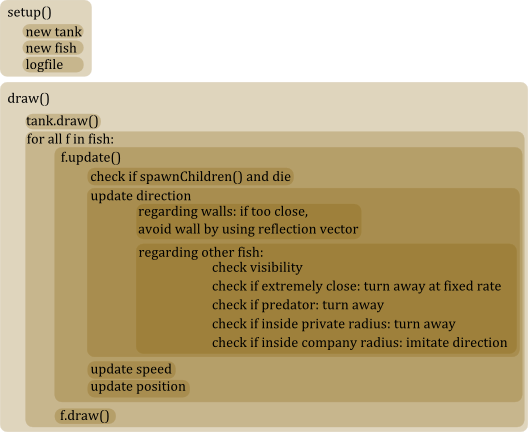
\includegraphics[width=\textwidth]{implementationsketch}
        \caption{Essential structure of the program}
        
\end{figure}

\subsection{Exporting the Values}
How I would translate that into something textile, I was not so sure at first, but I started with a thread-based idea, where each thread is seen as an individual. Macramé and Embroidery were favored candidates.

To be able to extract all important positions and values from the program I implemented several logging methods. The program produces a simple text-file, where the parameter values are noted as well as the positions of the fish (original coordinates plus coordinates scaled to fit the textile application), their id and their children. The tank class produces an image where the positions of the fish are noted pixelwise, the image shows their complete movement. I also export an SVG-file with a straight line connecting the end position of each fish with their children. This export can be done with additional text output directly within the SVG-file (the id of each fish above its "grave").

[TODO examples of the 3 log files]

\subsection{Parameters and Variations} % + Observations + Images}
There are several more, but some of the most important fish parameters/properties are:
[TODO detailed description]
- privateRadius
- companyRadius
- interpolationSpeed (speed of turns)
- timetoSpawn
- spawnAnglesDegree

These are the parameters I varied while observing the changes in the resulting image.
Figure [TODO] shows the outcomes for certain values.

- 30 privateRadius: 20 30 40 50
- 70 companyRadius: 50 70 90 120
- 100 interpolationSpeed (speed of turns) /ms: 50 100 150 200 250 350
- 6000 timetoSpawn: 3000 4000 5000 6000 8000 ms
- 135 spawnAnglesDegree +/- 0 10 20 45 70 90 135 180

\section{Textile Implementation}

\subsection{Textile Piece I}
\subsubsection{Method and Tools}

%TODO logfile
For 7 generations of fish, each having 2 children I need 2 hoch 7 threads (128). , for the piece I needes 16 strings of this cotton wool - which is quite thick. I tried to fit it through one "grid point" - even when I succeeded the accuracy of the grid was physically compromised, so I decided to at least ... for the first (or even the second) generation. The start point for the fish is 50/50, after dividing the thick cord into 4 subcords à 4 strings the start points are 51/50, 49/50, 50/49, 50/51.\\

\begin{minipage}[t]{0.48\textwidth}
    \raisebox{-0.9\totalheight}{\includegraphics[width=\textwidth]{stoffraster}}
    \captionof{figure}{Base material as canvas}
\end{minipage}
\hspace{0.5cm}
\begin{minipage}[t]{0.48\textwidth}
    For my first practical trial run I used evenweave with approximately 2mm per unit. To limit the size I scaled down the computed positions to fit a 100 by 100 grid (resulting in appr. 20cm by 20cm for the finished piece). The yellow thread was used as a counting help.
\end{minipage}
\vspace{0.5cm}

\begin{minipage}[t]{0.48\textwidth}
    \raisebox{-0.9\totalheight}{\includegraphics[width=\textwidth]{fadendetail}}
	\captionof{figure}{Applied material}
\end{minipage}
\hspace{0.5cm}
\begin{minipage}[t]{0.48\textwidth}
	Because my generations of fish are based on the number 2, I also need thread based on number 2. So I used cotton wool threads each already containing 8 ($=2^3$) sub-threads when feazed.\\
	To be able to manage the threads and associate them with one fish id I simply attached some paper to the string groups.
\end{minipage}
\vspace{0.5cm}

\subsection{Textile Piece II}
\subsubsection{Method and Tools}

\section{}
\section{}
\subsection{}

%\begin{figure}[h]
%        \centering
%        \begin{subfigure}[b]{0.31\textwidth}
%                %\includegraphics[width=\textwidth]{dist1}
%        \end{subfigure}
%        \begin{subfigure}[b]{0.31\textwidth}
%                %\includegraphics[width=\textwidth]{dist2}
%        \end{subfigure}
%        %\caption{Visualization of the projective distorted points}
%\end{figure}


Trial/Error runs? Unused parameters?

First (implemented) sketched out idea:

-	(explain main mechanism: finding the direction vector in each step, no randomness involved)
-	Other alterations/ playing with ideas: start with one fish that can spawn children (keep on moving or die after spawning)

Intermediate result:
-	Tracking positions in pixels : image with traces on picture (pixels, not lines)
-	Image with connecting lines (data = lines)

Role of Textiles in this?
-	Threads/knots as small part with defined behaviour (1. idea)
-	Errors over time, two tanks with same starting population grow apart (2. Idea, did not quite work, funny because with handcraft that happens : no identical pieces)
-	Connections to ancestors (3. Idea, without predators)
-	Connections to ancestors should limit the "life" of the  fish somehow (3. idea) : threads also limited, no infinite resource in real life, limited freedom?
-	-> include death somehow? Maybe the thread becomes limited depending on how close you were when your ancestor died : shorter thread?
-	New connections to fish you are close to for a longer time : frienships/partnerships (different color/weight?)
Textile finished piece:
-	Embroidery: pixelated image to threaded image (boring)
-	Connections to threaded image(series) (better? Development of generations)
-	Tree (knots/perls? = fish, length of edge is also determined by fish-bowl-movement) / graph : flexible

%----------------------------------------------------------------------------------------------------

%====================================================================================================
\newpage
\section*{Code}

%put the code here:
%\begin{lstlisting}
%\end{lstlisting}

%\bibliographystyle{plain}
%\bibliography{references}
\end{document}

